\section{Evaluation}
\label{sec:evaluation}

In this section, we performed several experiments to characterize such an ultrasound localization system. Most of the experiments are done in DOP center at Cory Hall, with a Macbook Pro as ultrasound transmitter and Samsung GALAXY S III phone (Android 4.1) running our application as the receiver.

\subsection{Power Consumption}
\label{sec:power-consumption}
We measured the power consumption of our application using LG Revolution VS910 with Android 2.3.4  (in this case, we used an experiment phone due to the potential risks). The summarized measured results are in Table.\,\ref{tab:power}. We could easily find out that having this application running in the background doesn't affect much of the power consumption. As for the case that the application runs in front, since there are a lot of screen drawings on the UI update events (either display the spectrum or the map), the application apparently burdens the battery, with an increase of about 59.8\% power consumption than usual.

Since there are so many factors which could potentially influence the power consumption, the measurement is mostly for rough estimation. But one interesting thing that we do observe by measuring the power consumption is that, a large portion of the power is used for screen, and more than 100mA current is usually used for radio and communication (there is occasional peaks when the screen is off). 

\begin{table}
  \centering
  \begin{tabular}{|l|c|c|}
    \hline
    & mean (mA) & standard variance (mA) \\
    \hline
    no app, screen on &  214.9 & 43.6 \\
    no app, screen off &  72.4 & 48.0 \\
    \hline
    app runs, screen on &  342.0 & 43.6 \\
    app runs {\em (background)}, screen on & 211.0 & 10.0 \\
    app runs {\em (background)}, screen off &  56.5 & 49.5 \\
    \hline
  \end{tabular}
  \caption{Power consumption of the application}
  \label{tab:power}
\end{table}


% screen on mean: 0.2149 var: 0.0019 -> 0.0436
% screen off mean: 0.0724 var: 0.0023 -> 0.0480
% % Screen on: 0.3256 0.1948 0.3563 0.2035 0.2110 0.1878 0.1874 0.1867 0.2207 0.2261 0.2135 0.2041 0.2014 0.1888 0.1893 0.1888 0.1882 0.1897 0.1913 0.1873 0.2036 0.1968 0.2691 0.2453 lab
% % Dim: 0.1854
% % Screen off: 0.0818 0.0318 0.0099 0.0833 0.0497 0.0062 
% % 0.0051 0.0037 0.0050 0.0041 0.0071 0.1202 0.1035 0.1232 0.0060 0.0052 0.1046 0.0905 0.0317 0.1014 0.0909 0.1588 0.1700 0.0836 0.0965 0.0924 0.1064 0.0568 0.0951 0.0900 0.0766 0.1246 0.0900 0.1034 0.0145 0.0059 0.0550 0.0451 0.0898 0.1050

% Running application
% screen on mean: 0.3420 var: 0.0027 -> 0.0520 
% screen on background mean: 0.2110 var: 0.0001 -> 0.01
% screen off background mean: 0.0565 var: 0.0024 -> 0.0495
% % Screen on: 0.2248 0.2379  0.2325     0.3312 0.3529 0.3512 0.3686 0.3519 0.4118 0.3416 0.3504 0.3339 0.3298 0.3499 0.3162 0.3495 0.3649 0.3471 0.3269 0.3626 0.3561  0.3585 0.3570 0.3495 0.3355 0.3749 0.3629 0.2559 0.4544 0.3623 0.3545 0.4343 0.4395 0.3946 0.3798 0.3525 0.3433 0.3490 0.3696 0.3338 0.3635 0.3433 0.3695 0.3141 0.3861 0.3173 0.3707 0.3736 0.4577 0.3371 0.3577 0.3421 0.3356 0.3393 0.3387 0.3484 0.3566 0.3178 0.3536 0.3573 0.3297 0.3238 0.2341 0.2349 0.2621 0.3493 0.3477 0.3499 0.3412 0.3438 0.3565 0.3502 0.3403 0.3599 0.3514 0.3402 0.3530 0.3416 0.3330 0.3690 0.3484 0.3600 0.2275 0.2181 0.2460 0.2364 0.2379 0.2623 0.3735 0.3502 0.4430 0.4042 0.4276 0.4293 0.3523 0.3373 0.3593 0.3107 0.3767 0.4200 0.3066 0.2086  
% % background screen on
% 0.2136 0.1883 0.2018 0.1941 0.1909 0.1907 0.1880 0.1924 0.1881 0.2056 0.1877 0.2001 0.2554 0.2251 0.2787 0.2756 
% % background screen off
% 0.0769 0.0649 0.0698 0.1014 0.0225 0.0077 0.0047 0.0045 0.0127 0.0043 0.0041 0.0350 0.1009 0.1676 0.0726 0.1196 0.0905 


\subsection{Signal Strength}
\label{sec:signal-strength}
We measure the received signal strength of signals in different frequencies. The maximum output sound level from our Macbook generator is 86$\sim$90dB. Since we have converted the received signal to frequency domain using FFT, the results are only relative values for the purpose of illustration of ultrasound's characteristics. The obtained figure is shown in Fig.\,\ref{fig:strength}, where we tested four different frequency points. Our distance parameter ranges from 20 inches to 140 inches. This experiment is done in Room 545K, whose length is around 150 inches. 

This figure shows that generally the received ultrasound signal is attenuating with the increase of distance. There might exist several points where the received signal strength is larger than those who are nearer; this is mainly caused by all kinds of reflection inside this room. Another observation is that with the increase of signal frequency, the signal strength is decreasing due to the imperfect frequency response of most microphones used in smartphones, but these signals are still large enough to be differentiated  from the noise.

\begin{figure}
  \centering
  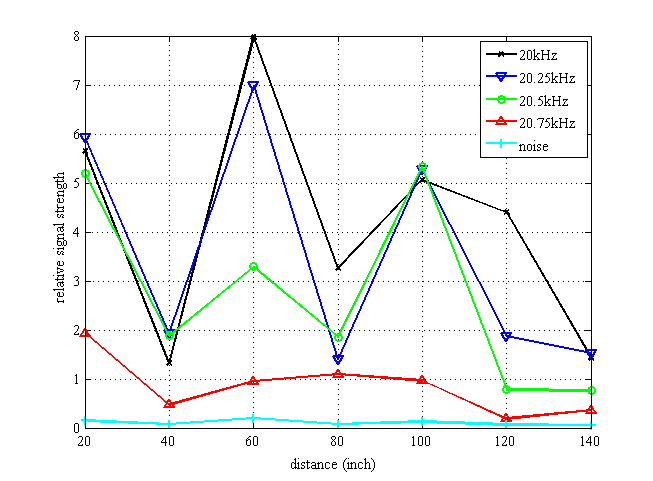
\includegraphics[width=0.9\columnwidth]{result_distance.png}
  \caption{Signal Strength vs. Distance}
  \vspace{-0.3cm}
  \label{fig:strength}
\end{figure}

\subsection{Obstacle Blocking}
\label{sec:obstacle-blocking}
As we have argued in Sec.\,\ref{sec:introduction} that the ultrasound can be easily reflected inside a room while the wall can be the perfect deliminator of spaces. In this section, we describes the experiment of validating such idea by measuring both the signal strength and the accuracy. We place the phone on both side of the glass wall of Room 545K, and run this application both for more than 1 minute.

The measurement of received signal after FFT operation is shown in Fig.\,\ref{fig:wallblock}. It's clearly attenuated after the blocking of the wall. We then calculate the detected results (the ground-truth in this case is 10110000). In the ``inside'' experiment, mostly the phone can correctly detect the room ID, with an accuracy of 96.06\% (it's 91.25\% before the filtering); while in the ``outside'' experiment, the detection always outputs 0.

\begin{figure}
  \centering
  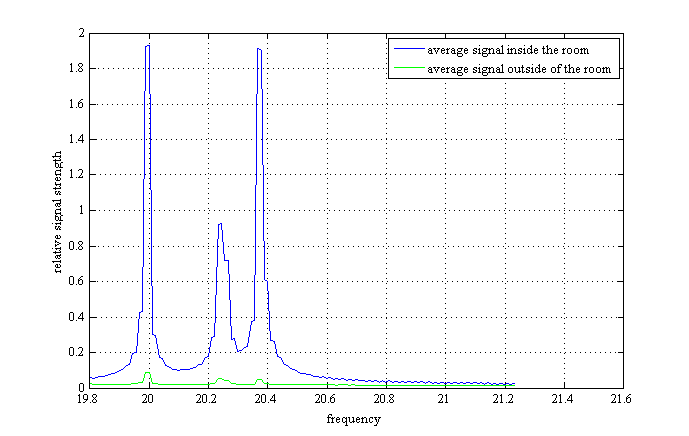
\includegraphics[width=0.9\columnwidth]{WallBlocking}
  \vspace{-0.3cm}
  \caption{The effect of wall blocking}
  \label{fig:wallblock}
\end{figure}

\subsection{Room Coverage}
\label{sec:room-coverage}
In the last section, we examined the effect of walls which will block the signal easily, and therefore the signal should be bouncing back and forth inside the room to create a fully coverage. We did experiment about such coverage characteristics by measuring eight different points inside the room. We compare the detected results with the ground-truth (both before and after filtering) and visualize the related accuracy in Fig.\,\ref{fig:coverage}. And from the result we could see that the ultrasound signal covers the entire room, and works pretty well for corner-cases. 

\begin{figure}
  \centering
  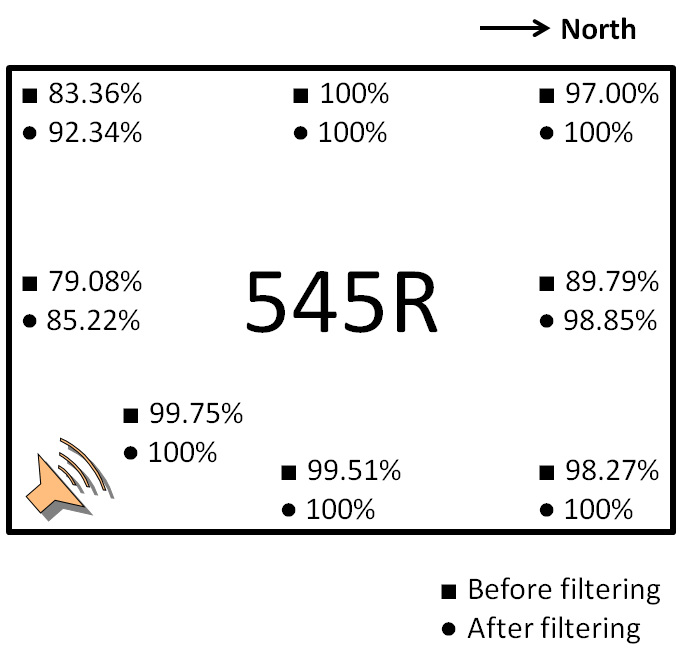
\includegraphics[width=0.6\columnwidth]{545R.png}
  \vspace{-0.3cm}
  \caption{Room coverage experiment}
  \label{fig:coverage}
\end{figure}

\subsection{Noise Resistance}
\label{sec:noise-resistance}
Another great feature we utilize about ultrasound is its noise resistance. Since talking, playing music and walking will not generate much signal that exceed 20kHz, such an ultrasound-based beacon should be able to resist noise pretty well. In order validate such idea of noise resistance, we need to know how it performs with the existence of different kinds of noise (such as speaking, coughing, music, etc.). 

The experiment result is shown in Table.\,\ref{tab:noiseres}, and it's clear that most human activity won't affect the detection too much. Clapping does affect this since they contains high frequency signals. But this will only affect a lot when clapping is continued with large volumne and for a long time, otherwise such noise will be removed by the exponential averaging filter.
\begin{table}
  \centering
  \begin{tabular}{|l|c|c|}
    \hline
    noise source & accuracy (before filtering) & accuracy (after filtering) \\
    \hline
    speaking &  99.93\% & 100\% \\
    music  &  94.44\% & 100\% \\
    coughing & 97.25\% & 100\% \\
    clapping & 69.17\% & 74.58\% \\
    walking & 100\% & 100\% \\
    \hline
  \end{tabular}
  \caption{Noise resistance characteristics}
  \label{tab:noiseres}
\end{table}

\subsection{Reception Rate}
\label{sec:reception-rate}
In this experiment, we plan to examine the overall detection of our algorithm. Since there are multipath effects, other kinds of noises, and maybe users' movement, the data reception rate will not be perfect. Our exponential moving average algorithm (in Sec.\,\ref{sec:android-application}) is used to cope with these imperfections, and its effectiveness has been demonstrated in each seperated experiment.

We run our application for 2 mins continously to collect the raw detected results and the filtered results in normal environment (phone holder moves around naturally during this experiment with all kinds of noises). The result is shown in Fig.\,\ref{fig:reception}, where we cluster the detected results using the histogram to illustrate the errors. The groundtruth room ID is 176, and the signal is successfully detected most of the time. Bit errors do happen occasionally; from our experiment, the overall reception rate is 67.60\%. After the filtering, some sporadic errors are corrected, and the overall detection has been improved to 87.50\%. 

Further observation reveals that most of the wrong detection resulted in Room ID 0, which means no reliable signal at all. We could just infer users' location as the previous room since it's not physically feasible of changing room that rapidly; such semantic combination of detected results with real scenario consideration will yield 97.25\% accuracy.

\begin{figure}
  \centering
  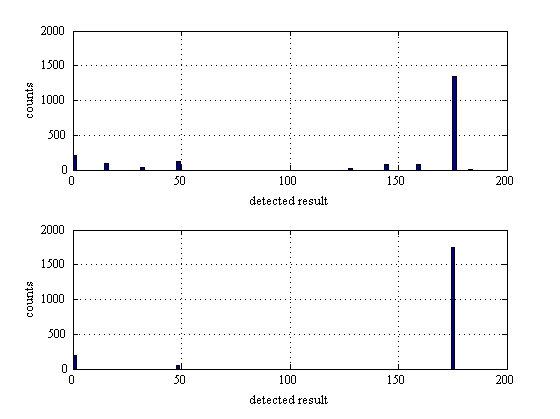
\includegraphics[width=0.9\columnwidth]{ReceptionRate}
  \caption{Histogram of the raw detected room ID ({\em up}); histogram of filtered result ({\em down})}
  \vspace{-0.3cm}
  \label{fig:reception}
\end{figure}




%% Master
%%% Local Variables: 
%%% mode: latex
%%% TeX-master: "ee149"
%%% End: 
